\section{Path Calculation}


\subsection{Positioning}


\frame
{
\frametitle{Sensor Types}

\begin{itemize}
\item Absolute sensors
	\begin{itemize}
	\item Lateration
		\begin{itemize}
		\item GPS
		\item Mobile telephony
		\end{itemize}
	\item Environment detection
		\begin{itemize}
		\item Image recognition
		\item Bumper, distance sensoro
		\end{itemize}
	\item Relative sensors
		\begin{itemize}
		\item Gyro, acceleration, magnetometer
		\item Rotary encoder
		\item Mouse sensor
		\end{itemize}
	\end{itemize}
\end{itemize}
}


\frame
{
\frametitle{Measure failures}

\begin{itemize}
\item Methodical
	\begin{itemize}
	\item Wrong calibration
	\item Wrong filter algorithm
	\end{itemize}
\item Randomly
\item Runaway value
\end{itemize}
}


\frame
{
\frametitle{Measure failures}
\makebox[\textwidth][c]{
\resizebox{0.75\textwidth}{!}{
\makebox[\linewidth]{
\pgfmathsetmacro{\drawSize}{0.65}

\newcommand*{\drawDart}[2]{
	\providelength{\dartCurrentSize}
	\setlength{\dartCurrentSize}{#1}
	\provideboolean{dartColor}
	\setboolean{dartColor}{true}
	\whiledo {\dartCurrentSize > 0}
	{
		\ifdartColor
			\path[fill=blue,draw=black] (0,0) circle (\dartCurrentSize);
		\else
			\path[fill=gray,draw=black] (0,0) circle (\dartCurrentSize);
		\fi
		\addtolength{\dartCurrentSize}{-#2}
		\setboolean{dartColor}{\ifdartColor false\else true\fi}
	}
 }

\newcommand*{\calcRealPos}[1]{
	\FPmul\pos{#1}{\drawSize}
}

\newcommand*{\drawFixDart}{
	\calcRealPos{3}
	\FPmul\partSize{\pos}{0.10}
	\drawDart{\pos cm}{\partSize cm}
}

\newcommand{\calcRandCirclePos}{
	\loop
		\pgfmathsetmacro{\posx}{rand}
		\pgfmathsetmacro{\posy}{rand}
		\FPmul\squarex{\posx}{\posx}
		\FPmul\squarey{\posy}{\posy}
		\FPadd\squaresum{\squarex}{\squarey}
		\ifdim \squaresum pt > 1pt
	\repeat
}

\newcommand{\drawPoint}[2]{
	\calcRealPos{#1}
	\pgfmathsetmacro{\posx}{\pos}
	\calcRealPos{#2}
	\path[draw=yellow] (\posx cm,\pos cm) circle (0.1cm);
}

\begin{tikzpicture}
\drawFixDart
\providecounter{ct}
\pgfmathsetseed{1}
\forloop{ct}{0}{\value{ct} < 30}{
	\calcRandCirclePos
	\FPmul\posx{\posx}{0.5}
	\FPmul\posy{\posy}{0.5}
	\drawPoint{\posx}{\posy}
}
\end{tikzpicture}

\begin{tikzpicture}
\drawFixDart
\providecounter{ct}
\forloop{ct}{0}{\value{ct} < 70}{
	\calcRandCirclePos
	\FPmul\posx{\posx}{2}
	\FPmul\posy{\posy}{2}
	\drawPoint{\posx}{\posy}
}
\end{tikzpicture}

\begin{tikzpicture}
\drawFixDart
\providecounter{ct}
\forloop{ct}{0}{\value{ct} < 70}{
	\calcRandCirclePos
	\FPmul\posx{\posx}{0.5}
	\FPadd\posx{\posx}{1}
	\FPmul\posy{\posy}{0.5}
	\FPadd\posy{\posy}{0.7}
	\drawPoint{\posx}{\posy}
}
\end{tikzpicture}

\begin{tikzpicture}
\drawFixDart
\providecounter{ct}
\forloop{ct}{0}{\value{ct} < 70}{
	\calcRandCirclePos
	\FPmul\posx{\posx}{0.5}
	\FPmul\posy{\posy}{0.5}
	\drawPoint{\posx}{\posy}
}
\drawPoint{2}{2}
\calcRealPos{3.1} \pgfmathsetmacro{\posfromx}{\pos}
\calcRealPos{3.1} \pgfmathsetmacro{\posfromy}{\pos}
\calcRealPos{2.1} \pgfmathsetmacro{\postox}{\pos}
\calcRealPos{2.1} \pgfmathsetmacro{\postoy}{\pos}
\draw[->, line width=2pt,color=red] (\posfromx,\posfromy) -- (\postox,\postoy);
\drawPoint{-1}{2.5}
\calcRealPos{-2.1} \pgfmathsetmacro{\posfromx}{\pos}
\calcRealPos{3.6} \pgfmathsetmacro{\posfromy}{\pos}
\calcRealPos{-1.1} \pgfmathsetmacro{\postox}{\pos}
\calcRealPos{2.6} \pgfmathsetmacro{\postoy}{\pos}
\draw[->, line width=2pt,color=red] (\posfromx,\posfromy) -- (\postox,\postoy);
\end{tikzpicture}
}
}
}
}


\frame
{
\frametitle{Combine different sensor}

\begin{itemize}
\item Algorithm have to ake care about
	\begin{itemize}
	\item Weight of sensor
	\item Type of sensor
	\item Measure fault type
	\item Precision
	\item Calibration
	\item Adapted filters
	\item ...
	\end{itemize}
\end{itemize}
}


\frame
{
\frametitle{Position specification}

\begin{itemize}
\item Stored
	\begin{itemize}
	\item Position + direction
		\begin{itemize}
		\item 2D
		\item 3D
		\end{itemize}
	\item Particle Cloud
		\begin{itemize}
		\item Probability
		\end{itemize}
	\end{itemize}
\item Related to
	\begin{itemize}
	\item Start point
	\item Objects (Barriers)
	\end{itemize}
\end{itemize}
}


\frame
{
\frametitle{Position specification}
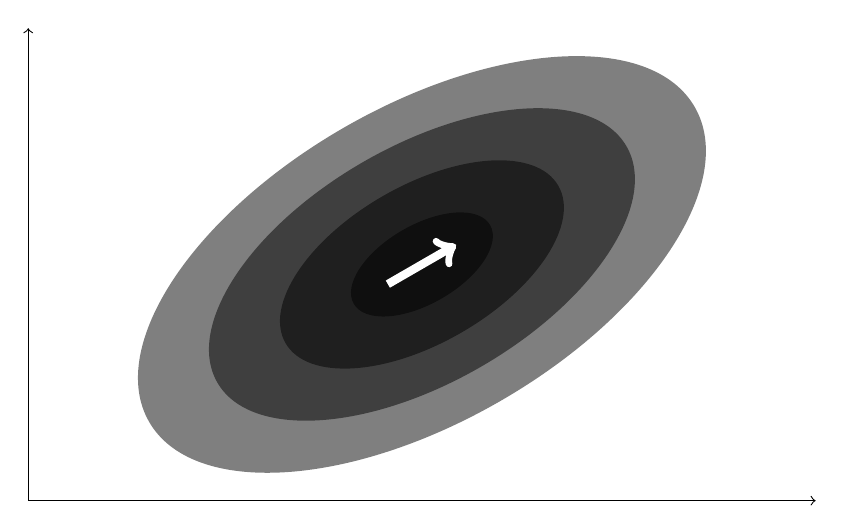
\begin{tikzpicture}
	\draw[->] (0,0) -- (10,0);
	\draw[->] (0,0) -- (0,6);
	\begin{scope}[shift={(5,3)},rotate=30]
		\foreach \x in {0,0.5,...,2}{
			\fill  [fill=black, semitransparent] (0,0) ellipse ({2 * \x} and {\x});
		}
		\draw[->,color=white,line width=3pt] (-0.5,0) -- +(1,0);
	\end{scope}
\end{tikzpicture}

}
